\section{Motivation}
\label{sec:supportingintlangs}

\begin{itemize}
  \item Building a symbex engine for high-level languages is hard engineering.
\end{itemize}

language is even harder.  A symbolic execution engine has to map language elements to manipulations of the symbolic execution state, and is thus essentially a ``symbolic interpreter'' for the language.  Complete support of a modern dynamic language with features such as exceptions and reflection prevents cutting any corners and requires to replicate almost all functionality of the original interpreter. Conceptually, exploring multiple paths by symbolic execution is a generalization of executing a single path, which already requires a full interpreter.
%
Building a correct and complete symbolic execution engine for an interpreted language is generally harder than building one for a low-level language. 
%
Statements of interpreted languages can wrap complex operations that, in lower-level languages, would be implemented through libraries. For instance, Python strings are a built-in type offering more than 30 operations (such as \codebit{find}) as part of the language, implemented natively in the interpreter. 
%
Other language features that allow to inspect or even modify the code itself, i.e., runtime reflection, are even more tedious to implement and very hard to get right.

Finally, besides requiring an enormous initial effort to build a symbolic execution engine that fully supports them, dynamic languages also evolve fast. This implies constant, labor-intensive maintenance and co-evolution of the symbolic execution engine, if it is to keep up with the newest versions of the language.

%%%%%%%%%%%%%%%%%%%%%%%%%%%%%%%%%%%%%%%%%%%%%%%%%%%%%%%%%%%%%%%%%%%%%%%%%%%%%%%%

\section{Symbolically Executing the Interpreter}

\begin{itemize}
\item We can use the interpreter as ``executable language specs'' by plugging it into a low-level (e.g., binary) symbolic execution engine.
\item However, this won't work out of the box.
\end{itemize}

Considering the difficulty of directly supporting interpreted languages, we resort to symbolically executing the interpreter itself, since it completely defines the semantics of the target language as a function of the semantics of the language the interpreter is implemented in.
%
After compiling the interpreter to a format supported by an existing symbolic execution engine, one can symbolically execute an interpreted program by symbolically executing the interpreter with the target program as argument.
%
However, even though in principle this direct approach yields a symbolic execution engine for the target language, it is impractical, due to the engine not being aware of the control flow of the interpreted program.

\paragraph{High- vs. Low-level Program Paths}

\begin{figure}
  \centering
  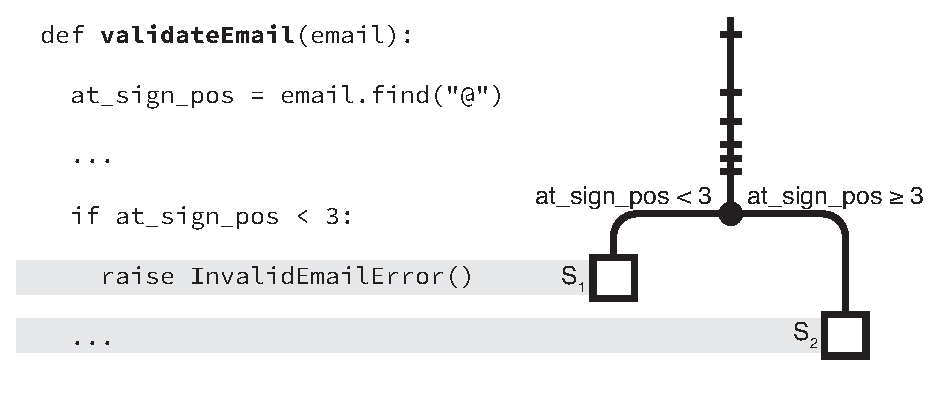
\includegraphics[width=2.2in]{figures/chef/running-example}
  \caption{Two examples of Python code that lead to path explosion when the interpreter running it is symbolically executed.}
  \label{fig:running-examples}
\end{figure}


An interpreted program conceptually executes both on a high level---the level of the target language---and a low level---the level of the interpreter.
%
A high-level program path is a sequence of values of the high-level program counter (\hlpc). Each \hlpc value corresponds to a program statement or bytecode instruction (both Python and Lua use intermediate bytecode).  Branches can occur explicitly at control flow statements, or implicitly through exceptions.
%
A low-level program path is a sequence of machine instructions from the interpreter binary, including its code for internal bookkeeping (e.g., details of reference counting and garbage collection).

Due to the additional implementation details, a single high-level path can map to multiple low-level paths.
%
Figure~\ref{fig:running-examples} shows two examples of Python code that have few high-level but many low-level paths. The \codebit{validateEmail} method has only two high-level paths, but its use of \codebit{string.find} leads to as many low-level paths as there can be characters in the \codebit{email} string.
%
The second example \codebit{average} may come as more of a surprise: even though it has just a single high-level path, symbolic execution can end up enumerating many low-level paths: Python uses arbitrary-precision integers, so the interpreter may have to iterate over digit vectors of arbitrary length, which can in principle spawn arbitrarily many paths.


\paragraph{Challenges for Search Strategies}
%
The search strategy of a low-level symbolic execution engine is oblivious to the high-level program structure of the target program, and it essentially just tries to cover the interpreter. This generally leads to covering the same high-level paths many times with multiple distinct low-level paths.
%
For instance, a high-level statement like \codebit{find} can lead to hundreds of alternate states, whereas a primitive integer comparison might just create a single one. Therefore, the low-level search strategy is likely to explore multiple ways for \codebit{find} to succeed or fail, without increasing high-level coverage, before eventually exploring the alternate outcome of the comparison.

\begin{figure}
  \centering
  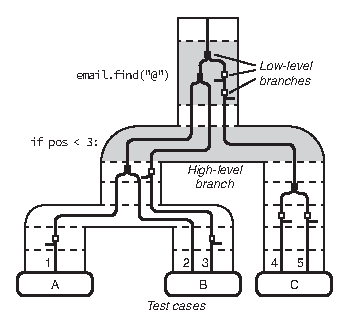
\includegraphics[width=2.8in]{figures/chef/hl-symbex}
  \caption{High-level execution tree (paths A, B, and C), as induced by its low-level execution paths (1--5) for the first running example in Figure~\ref{fig:running-examples}.  Dotted lines segment high-level execution paths into bytecode instructions.  One high-level path may correspond to multiple low-level paths explored.}
  \label{fig:hl-symbex}
\end{figure}

The key is to make the engine aware of the high-level interpreted program. By tracing the values of the \hlpc, the engine can construct a high-level control flow graph~(CFG) on the fly that can be be leveraged by the search strategy.

Alas, a strategy cannot straightforwardly determine future branching points in a high-level CFG: two low-level paths can fork from the same prefix \emph{before} their corresponding high-level paths do.  This can be due to having distinct bytecode instructions for comparisons and conditional jumps, or due to native library calls.  
%
In Figure~\ref{fig:hl-symbex}, three low-level paths fork within the single \hlpc location for \codebit{email.find}. The low-level paths remain on the same high-level path until reaching the branching \hlpc, where they diverge into two distinct high-level paths. The relevant alternate low-level states for covering the distinct high-level paths thus were located away from the location of the code interpreting the high-level control flow statement.
%
The issue of pre-determining branches is present also when exploring regular code, but it is ubiquitous when exploring code on interpreters.



We now present the architecture of \chef (Section~\ref{sec:architecture}) and introduce \cupa, our state selection mechanism (Section~\ref{sec:cupa}). We then describe \cupa optimized for exploring distinct high-level paths (Section~\ref{sec:cupa-paths}) and optimized for high line coverage~(Section~\ref{sec:cupa-coverage}).

\subsection{System Overview}
\label{sec:architecture}

\chef is a platform for language-specific symbolic execution. Provided with an interpreter environment, which acts as an executable language specification, it becomes a symbolic execution engine for the target language (see Figure~\ref{fig:system-arch}).
%
The resulting engine can be used like a hand-written one, in particular for test case generation. When fed with a target program and a symbolic test case (also called test driver or test specification in the literature), it outputs a set of concrete test cases, as shown in Figure~\ref{fig:system-arch}.

\begin{figure}
  \centering
  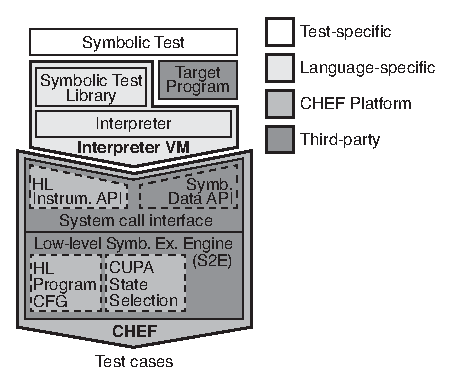
\includegraphics[width=2.6in]{figures/chef/system-arch}
  \caption{Schema of \chef's architecture.}
  \label{fig:system-arch}
\end{figure}

\chef is built on top of the S2E analysis platform~\cite{s2eSystem}. S2E symbolically executes a virtual machine containing the interpreter and a testing library at the level of machine code,  including the OS kernel, drivers, and user programs.  S2E provides an API that guest code can use to declare memory buffers as symbolic. Comparisons on symbolic values cause S2E to fork new paths, which are enqueued and explored following a search strategy.
%
\chef extends the S2E guest API with a high-level instruction instrumentation call (Section~\ref{sec:exposehlpc}), invoked by interpreters to trace the currently executing high-level path.  The explored high-level paths are used to construct a high-level execution tree and a low-level to high-level mapping (i.e., the data structure shown in Figure~\ref{fig:hl-symbex}).  \chef uses a state selection strategy to maximize the ratio of high-level to low-level paths (Section~\ref{sec:cupa}).

The resulting engine is a correct symbolic execution engine for the target language \textit{as defined by the interpreter}. It is fully precise and theoretically complete, i.e., it will not explore infeasible paths and will eventually explore all paths. The usual limitations of symbolic execution engines apply: completeness holds only under the assumption that the constraint solver can reason about all generated path conditions, and it is understood that exhaustive exploration is usually impossible in finite time.

%%%%%%%%%%%%%%%%%%%%%%%%%%%%%%%%%%%%%%%%%%%%%%%%%%%%%%%%%%%%%%%%%%%%%%%%%%%%%%%%

\section{High-level Symbolic Execution}
\begin{itemize}
\item Define the concept of high-level path.
\item Define the notion of high-level state.  Introduce the notion of completeness model, and discuss the tradeoffs between each.
\end{itemize}

%%%%%%%%%%%%%%%%%%%%%%%%%%%%%%%%%%%%%%%%%%%%%%%%%%%%%%%%%%%%%%%%%%%%%%%%%%%%%%%%

\section{High-level Control Flow Reconstruction}
\begin{itemize}
\item We need to bridge the gap between the stream of x86 instructions and stream of high-level instructions.
\item Manual approach: interpreter loop annotation.
\item Automated approach: use calibration program + look for memory access patterns inside the interpreter.
\end{itemize}

We now explain how to prepare an interpreter for \chef: the first and mandatory step is to instrument the main interpreter loop to report \hlpcs (Section~\ref{sec:exposehlpc}); the second and optional step is to optimize the interpreter for efficient symbolic execution (Section~\ref{sec:optimzeforsymbex}).  \chef provides an API (Table~\ref{tab:api}) that will be explained along with its use.  Finally, we discuss the remaining work of building a language-specific testing API to the resulting engine (Section~\ref{sec:testingAPI}).

\begin{table}
\centering
\small
\begin{tabular}{| l | l | }
\hline
\textbf{API Call} & \textbf{Description} \\
\hline
\codebit{log\_pc(pc, opcode)} & Log the interpreter PC and opcode \\
\hline
\codebit{start\_symbolic()} & Start the symbolic execution \\
\codebit{end\_symbolic()} & Terminate the symbolic state \\
\hline
\codebit{make\_symbolic(buf)} & Make buffer symbolic \\
\codebit{concretize(buf)} & Concretize buffer of bytes \\
\codebit{upper\_bound(value)} & Get maximum value for expression\\
                              & on current path \\
\codebit{is\_symbolic(buf)} & Check if buffer is symbolic \\
\codebit{assume(expr)} & Assume constraint \\
\hline
\end{tabular}
\caption{The \chef API used by the interpreters running inside the S2E VM.}
\label{tab:api}
\end{table}

To reconstruct the high-level program paths and CFG, \chef needs to identify the high-level instructions executed on each low-level path.  \chef provides the \codebit{log\_pc(pc, opcode)} API call to the interpreter, which declares the current high-level program location and the type (opcode) of the next instruction.  A high-level instruction is executed in between two consecutive \codebit{log\_pc} calls.
%
Interpreters typically contain a main interpretation loop that \codebit{switch}-es over the type of the current instruction and invokes specific handlers.  The \codebit{log\_pc} call can be added conveniently at the head of the interpreter loop.

In our design, we make minimal assumptions about the language structure, so the \hlpc and opcode values are opaque; the \cupa strategies were designed accordingly.  Nonetheless, more specific versions of the system could add structure to the two values, e.g. provide a pair of function name and offset as \hlpc.  The additional information can be used by \chef to improve the exploration heuristics (e.g., by creating a \cupa class).

The granularity of \codebit{log\_pc} calls depends on the language structure.  \chef's correctness does not depend on the specific instrumentation pattern, but the more closely the reported \hlpc corresponds to statements in the target program, the more accurately \cupa can cluster states. In the extreme, if \codebit{log\_pc} is never invoked, \chef would see the entire program as a single high-level instruction and lose the advantage of \cupa clustering for \hlpcs.

%%%%%%%%%%%%%%%%%%%%%%%%%%%%%%%%%%%%%%%%%%%%%%%%%%%%%%%%%%%%%%%%%%%%%%%%%%%%%%%%

\section{Interpreter Optimizations}
\label{sec:optimzeforsymbex}

\begin{itemize}
\item Goal: reduce path explosion in the interpreter.
\item Approach: ``anti-optimizations'' that slow down linear execution, but boost multi-path execution.
\item Hash neutralization.
\item String interning.
\item Handling memory allocations.
\end{itemize}

In order to maximize performance, interpreters make heavy use of special cases and sophisticated data structures.  Unfortunately, these features hurt the performance of symbolic execution by amplifying path explosion and increasing the complexity of symbolic formulas~\cite{overify}.

We identify a number of easy optimizations that preserve the interpretation semantics but significantly improve symbolic execution performance.  The optimizations use the \chef API in the last block of rows in Table~\ref{tab:api}.

\paragraph{Neutralizing Hash Functions}

Hash functions are especially common in interpreters, due to the internal use of hash tables for associative data structures (e.g., Python dictionaries or Lua tables).  However, they are generally a problem in symbolic execution: a symbolic value added to a hash table (a)~creates constraints that essentially ask the constraint solver to reverse a hash function, which is often hard, and (b)~causes the exploration to fork on each possible hash bucket the value could fall into.
%
A simple and effective optimization is to \emph{neutralize the hash function}, i.e., replace it with a degenerate one returning a single constant. This change honors the usual contracts for hash functions (equal objects have equal hashes) and will turn hash lookups into list traversals.

\paragraph{Avoiding Symbolic Pointers}

Input-dependent pointers (also referred to as symbolic pointers) may point to multiple locations in the program memory, so a pointer dereference operation would have to be resolved for each possible location.  In practice, symbolic execution engines deal with this situation in one of two ways:
%
(a)~fork the execution state for each possible concrete value the symbolic pointer can take; or
%
(b)~represent the dereference symbolically as a read operation from memory at a symbolic offset and let the constraint solver ``deal'' with it.
%
Both ways hurt symbolic execution, either by causing excessive path explosion or by burdening the constraint solver.

While there is no generic way to avoid symbolic pointers other than concretizing their values (the \codebit{concretize} API call) at the price of losing completeness, there are specific cases where they can be avoided.

First, \emph{the size of a buffer can be concretized} before allocation.  A symbolic size would most likely cause a symbolic pointer to be returned, since a memory allocator computes the location of a new block based on the requested size.  To avoid losing completeness, a symbolic execution-aware memory allocator can determine a (concrete) upper bound on the requested size and use that value for reserving space, while leaving the original size variable symbolic.  This way, memory accesses to the allocated block would not risk being out of bounds.  Figure~\ref{fig:sym-malloc} shows how the \chef API is used to wrap a call to the \codebit{malloc} function in the standard C library.

\begin{figure}
  \centering
  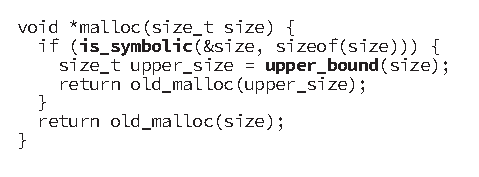
\includegraphics[width=2.6in]{figures/chef/mallocopt}
  \caption{Example of a symbolic execution-aware \codebit{malloc} function wrapper created using the \chef API.  If the allocation size is symbolic, the wrapper determines its upper bound and issues a concrete request to the underlying implementation.}
  \label{fig:sym-malloc}
\end{figure}

Second, \emph{caching and ``interning'' can be eliminated}.  Caching computed results and value interning (i.e., ensuring that a single copy of each possible value of a type is created) are common ways to improve the performance of interpreters.  Alas, when a particular value is computed, its location in memory becomes dependent on its value. If the value was already in the cache or in the interned store, it is returned from there, otherwise a new value is computed.  During symbolic execution, this logic becomes embedded in the value of the returned pointer, which becomes symbolic.  Disabling caching and interning may hurt the native performance of the program, but it can give a significant boost when running inside a symbolic execution engine.

\paragraph{Avoiding Fast Paths}

A common way to speed-up the native performance of a function is to handle different classes of inputs using faster specialized implementations (``fast paths'').  For example, a string comparison automatically returns false if the two strings have different lengths, without resorting to byte-wise comparison.

Fast paths may hurt symbolic execution because they cause symbolic branches in the code checking for the special input conditions.  \emph{Eliminating short-circuited returns} can reduce path explosion.  Instead of returning to the caller as soon as it produced an answer, the function continues running and stops on an input-independent condition.  For example, when comparing two strings of concrete length, a byte-wise string comparison would then traverse the entire string buffers in a single execution path, instead of returning after the first difference found.


\subsection{Testing API}
\label{sec:testingAPI}

Programs to be tested can be fed symbolic inputs by marking input buffers with \codebit{make\_symbolic} and defining conditions over the input with the \codebit{assume} call, in accordance to the test specification.  Note that the buffer is a memory region of concrete bounds.  It is the job of the symbolic test library in the interpreter VM to convert from the language data structures (e.g., strings, integers) to the memory locations used to store the data in the interpreter implementation.

%%% Local Variables: 
%%% mode: latex
%%% eval: (visual-line-mode)
%%% fill-column: 1000000
%%% TeX-master: "main"
%%% End:
